% Pontos A (0,0), B (1,0.75), C (2,1.5), D (3,0.75), E (4,0), F (2,0)
% Apoio móvel em A, apoio fixo em E.
% Viga em AB, BC, CD, DE, EF, FA, BF, DF, CF.
% Carga pontual de 10kN em B para baixo, 8kN em C para direita, 15kN em F para baixo

\documentclass[tikz]{standalone}
\usepackage{stanli}
\usetikzlibrary{calc}

\begin{document}
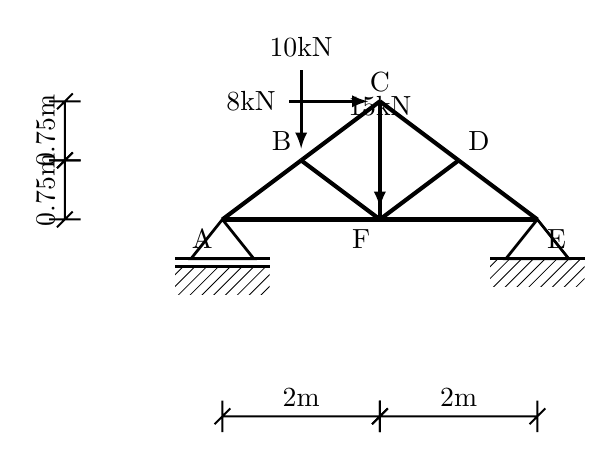
\begin{tikzpicture}
    % Definição dos pontos
    \point{A}{0}{0}
    \point{B}{1}{0.75}
    \point{C}{2}{1.5}
    \point{D}{3}{0.75}
    \point{E}{4}{0}
    \point{F}{2}{0}

    % Definição das vigas (barras da treliça/estrutura)
    \beam{2}{A}{B}
    \beam{2}{B}{C}
    \beam{2}{C}{D}
    \beam{2}{D}{E}
    \beam{2}{E}{F}
    \beam{2}{F}{A}
    \beam{2}{B}{F}
    \beam{2}{D}{F}
    \beam{2}{C}{F}

    % Apoios
    \support{2}{A} % Apoio móvel em A
    \support{1}{E} % Apoio fixo em E

    % Cargas pontuais
    % B: 10kN para baixo (90)
    \load{1}{B}[90]
    % C: 8kN para direita (180)
    \load{1}{C}[180]
    % F: 15kN para baixo (90)
    \load{1}{F}[90]

    % Notações de pontos
    \notation{1}{A}{A}[below left]
    \notation{1}{B}{B}[above left]
    \notation{1}{C}{C}[above]
    \notation{1}{D}{D}[above right]
    \notation{1}{E}{E}[below right]
    \notation{1}{F}{F}[below left]

    % Notações de cargas (seguindo as regras de offset)
    \notation{1}{B}{10kN}[above=12mm]
    \notation{1}{C}{8kN}[left=12mm]
    \notation{1}{F}{15kN}[above=12mm]

    % Dimensionamento Horizontal
    % Calculado para não sobrepor aos apoios (distância de -25mm)
    \dimensioning{1}{A}{F}{-25mm}[2m]
    \dimensioning{1}{F}{E}{-25mm}[2m]

    % Dimensionamento Vertical
    % À esquerda da estrutura
    \dimensioning{2}{A}{B}{-20mm}[0.75m]
    \dimensioning{2}{B}{C}{-20mm}[0.75m]

\end{tikzpicture}
\end{document}